\documentclass[12pt]{article}
\setlength{\oddsidemargin}{0in}
\setlength{\evensidemargin}{0in}
\setlength{\textwidth}{6.5in}
\setlength{\parindent}{0in}
\setlength{\parskip}{\baselineskip}
\usepackage{amsmath,amsfonts,amssymb}
\usepackage{graphicx}
\usepackage{enumitem}
\usepackage[]{algorithmicx}
\usepackage{amsthm}
\usepackage{fancyhdr}
\pagestyle{fancy}
\setlength{\headsep}{36pt}

\usepackage{hyperref}

\theoremstyle{remark}
\newtheorem*{solution}{Solution}

\newcommand{\makenonemptybox}[2]{%
%\par\nobreak\vspace{\ht\strutbox}\noindent
\item[]
\fbox{% added -2\fboxrule to specified width to avoid overfull hboxes
% and removed the -2\fboxsep from height specification (image not updated)
% because in MWE 2cm is should be height of contents excluding sep and frame
\parbox[c][#1][t]{\dimexpr\linewidth-2\fboxsep-2\fboxrule}{
  \hrule width \hsize height 0pt
  #2
 }%
}%
\par\vspace{\ht\strutbox}
}
\makeatother

\begin{document}

\lhead{{\bf CSCI 3104, Algorithms \\ Problem Set 3a (9 points)} }
\rhead{Name: Luna McBride \\ ID: 107607144 \\ {\bf Profs.\ Hoenigman \& Agrawal\\ Fall 2019, CU-Boulder}}
\renewcommand{\headrulewidth}{0.5pt}

\phantom{Test}

\begin{small}
\textbf{Instructions for submitting your solution}:
\vspace{-5mm} 

\begin{itemize}
	\item The solutions \textbf{should be typed} and we cannot accept hand-written solutions. \href{http://ece.uprm.edu/~caceros/latex/introduction.pdf}{Here's a short intro to Latex.}
	\item You should submit your work through \href{https://www.gradescope.com/courses/59294}{\textbf{Gradescope}} only.
	\item If you don't have an account on it, sign up for one using your CU email. You should have gotten an email to sign up. If your name based CU email doesn't work, try the identikey@colorado.edu version. 
	\item Gradescope will only accept \textbf{.pdf} files (except for code files that should be submitted separately on Gradescope if a problem set has them) and \textbf{try to fit your work in the box provided}. 
	\item You cannot submit a pdf which has less pages than what we provided you as Gradescope won't allow it. 
	\item Verbal reasoning is typically insufficient for full credit. Instead, write a logical argument, in the style of a mathematical proof.
	\item For every problem in this class, you must justify your answer:\ show how you arrived at it and why it is correct. If there are assumptions you need to make along the way, state those clearly.
	
	\item You may work with other students. However, \textbf{all solutions must be written independently and in your own words.} Referencing solutions of any sort is strictly prohibited. You must explicitly cite any sources, as well as any collaborators. 
\end{itemize}
\vspace{-4mm} 
\end{small}

\hrulefill

\newpage
\begin{enumerate}



\item Suppose we have a number of events $m_{i}$. Each event starts at time $s_{i}$ and finishes at time $e_{i}$, where $0 \leq s_{i} < e_{i}$. We represent the event $m_{i}$ with the closed interval $[s_{i}, e_{i}].$ Our goal is to construct a maximum size set of events, where no two events in the set overlap. \\

\noindent Suppose the following intervals are provided.
\begin{center}
\begin{tabular}{c|c}
Event Index & Interval \\ \hline
1 & $[1, 2]$ \\ 
2 & $[3, 4]$ \\
3 & $[5, 6]$ \\
4 & $[7, 8]$ \\
5 & $[0, 20]$.
\end{tabular}
\end{center}

\begin{enumerate}[label=(\alph*)]
\item (1 pt) What is the maximum size set of events that can be selected such that no two events in the set overlap? Include the list of the events selected in your answer.
\begin{solution}
$\newline \graphicspath{{C:\Users\Luna.DESKTOP-PEBO18O\Dropbox\CSCI3104}}$$ 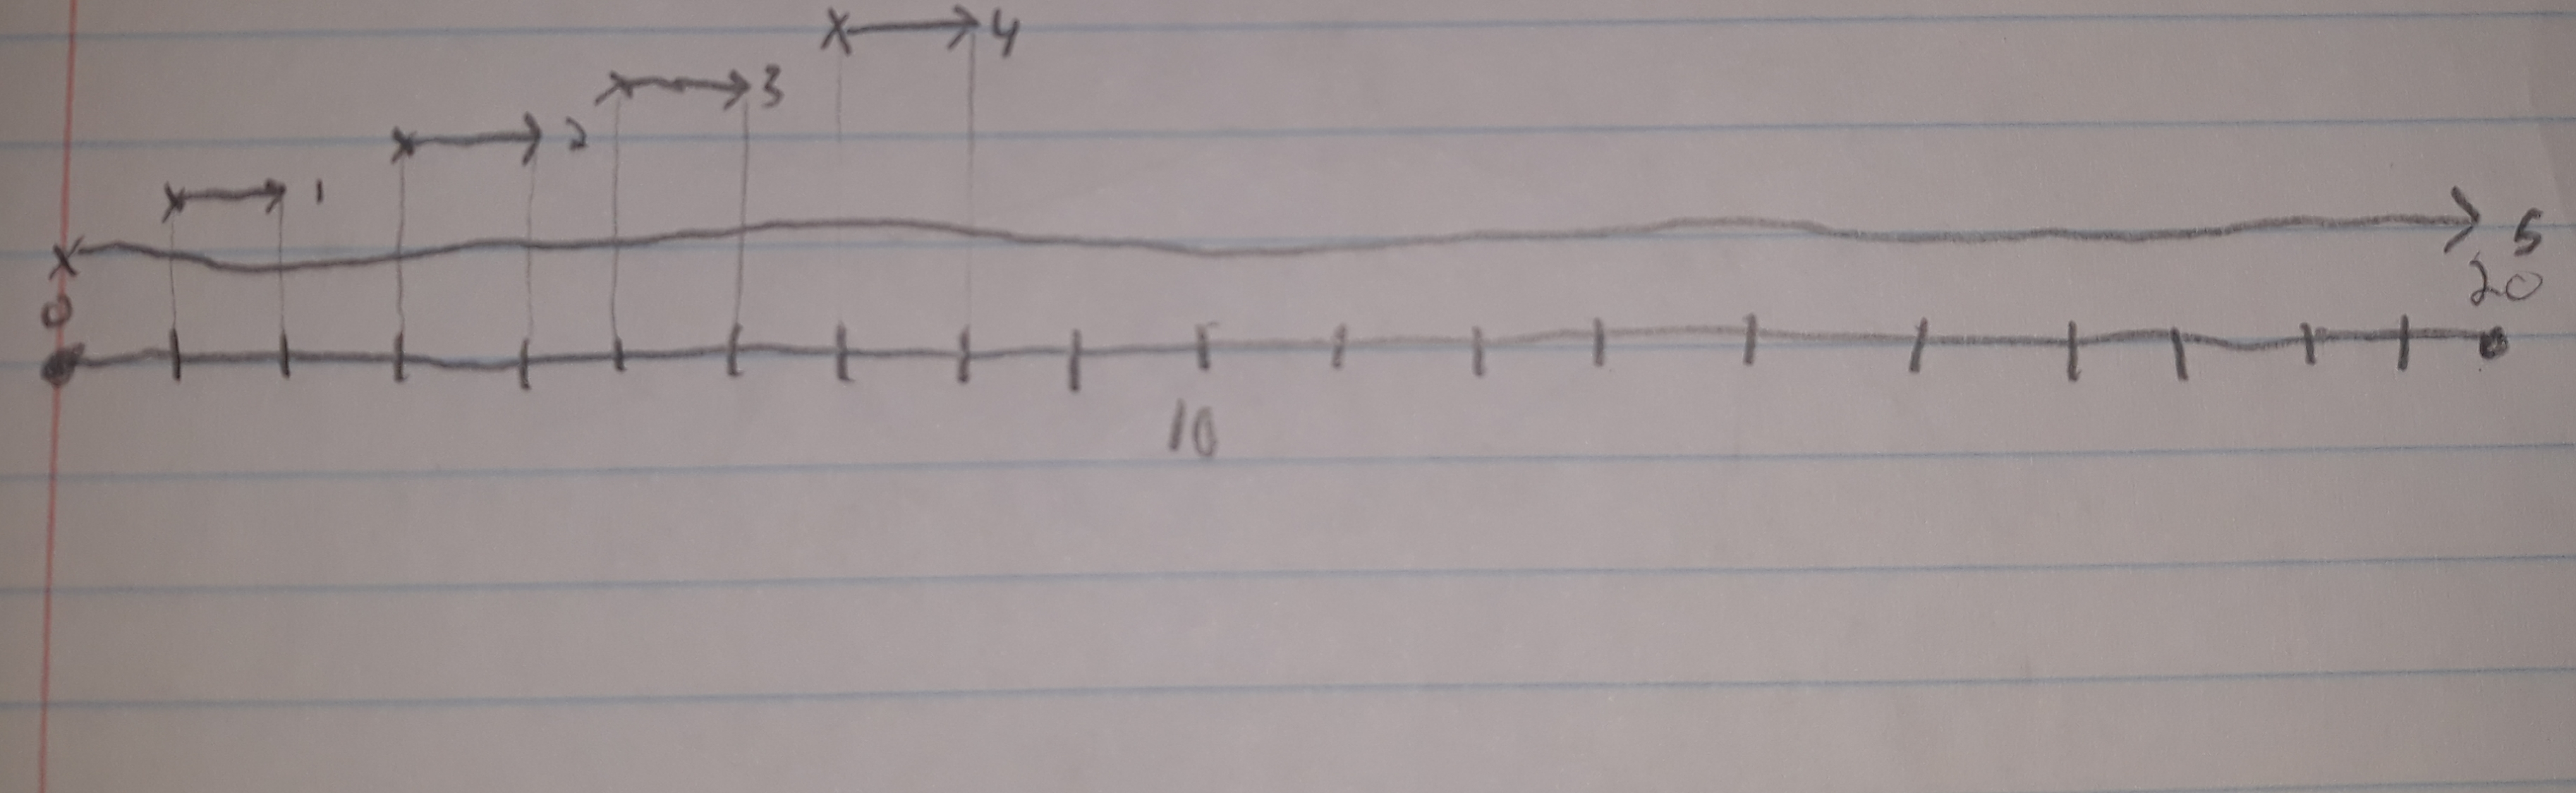
\includegraphics[width=\textwidth]{Graph} \newline \newline$ The 5th interval is in conflict with everything else and would take all the time, so we have to scrap it. $\newline \newline$ That leaves 4 non-overlapping events, being events (1 [1-2],2 [3-4],3 [5-6],4 [7-8])
\end{solution}

\newpage
\item (2 pt) Suppose we sort the intervals in ascending order by start time. Consider a greedy algorithm that selects the next event based on earliest start time, so long as the interval selected does not conflict with any previously selected interval. Using the intervals provided, show that this greedy algorithm fails to provide a maximum size set of events, where no two events in the set overlap. That is, the solution returned by this greedy algorithm is not optimal.
\begin{solution}

\end{solution}
$\newline 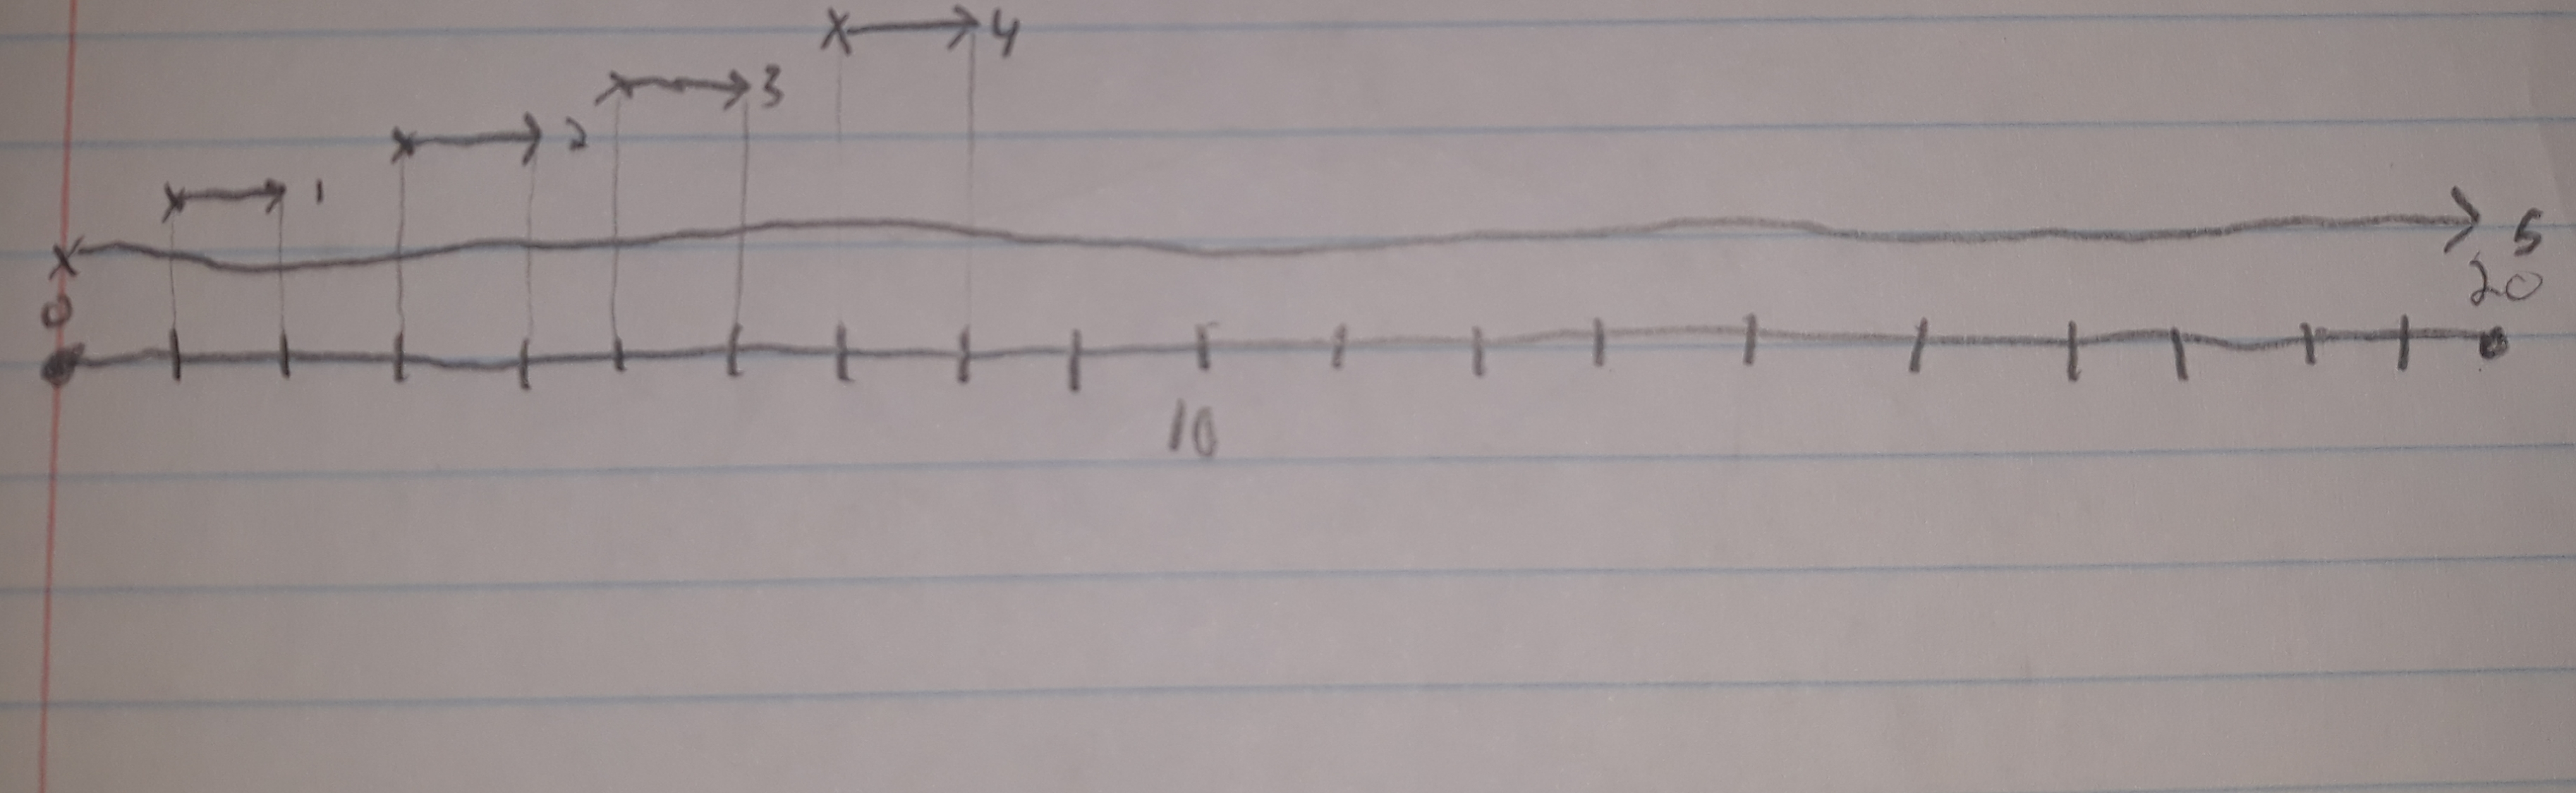
\includegraphics[width=\textwidth]{Graph} \newline$ (copied down here for convenience) $\newline \newline$ As shown in the graph, interval 5 ([0,20]) takes up all available times. However, since it is the earliest, it is picked. $\newline \newline$ This means the greedy algorithm only chooses 1 interval instead of the optimal 4, which is not optimal.
\end{enumerate}


\newpage
\item Using the same definition in Problem 1, suppose the following intervals are provided.
\begin{center}
\begin{tabular}{c|c}
Event Index & Interval \\ \hline
1 & $[1, 10]$ \\ 
2 & $[11, 20]$ \\
3 & $[21, 30]$ \\
4 & $[9, 12]$ \\
5 & $[19, 22]$.
\end{tabular}
\end{center}

\begin{enumerate}[label=(\alph*)]
\item (1 pt) What is the maximum size set of events that can be selected such that no two events in the set overlap? Include the list of the events selected in your answer.
\begin{solution}
$\newline 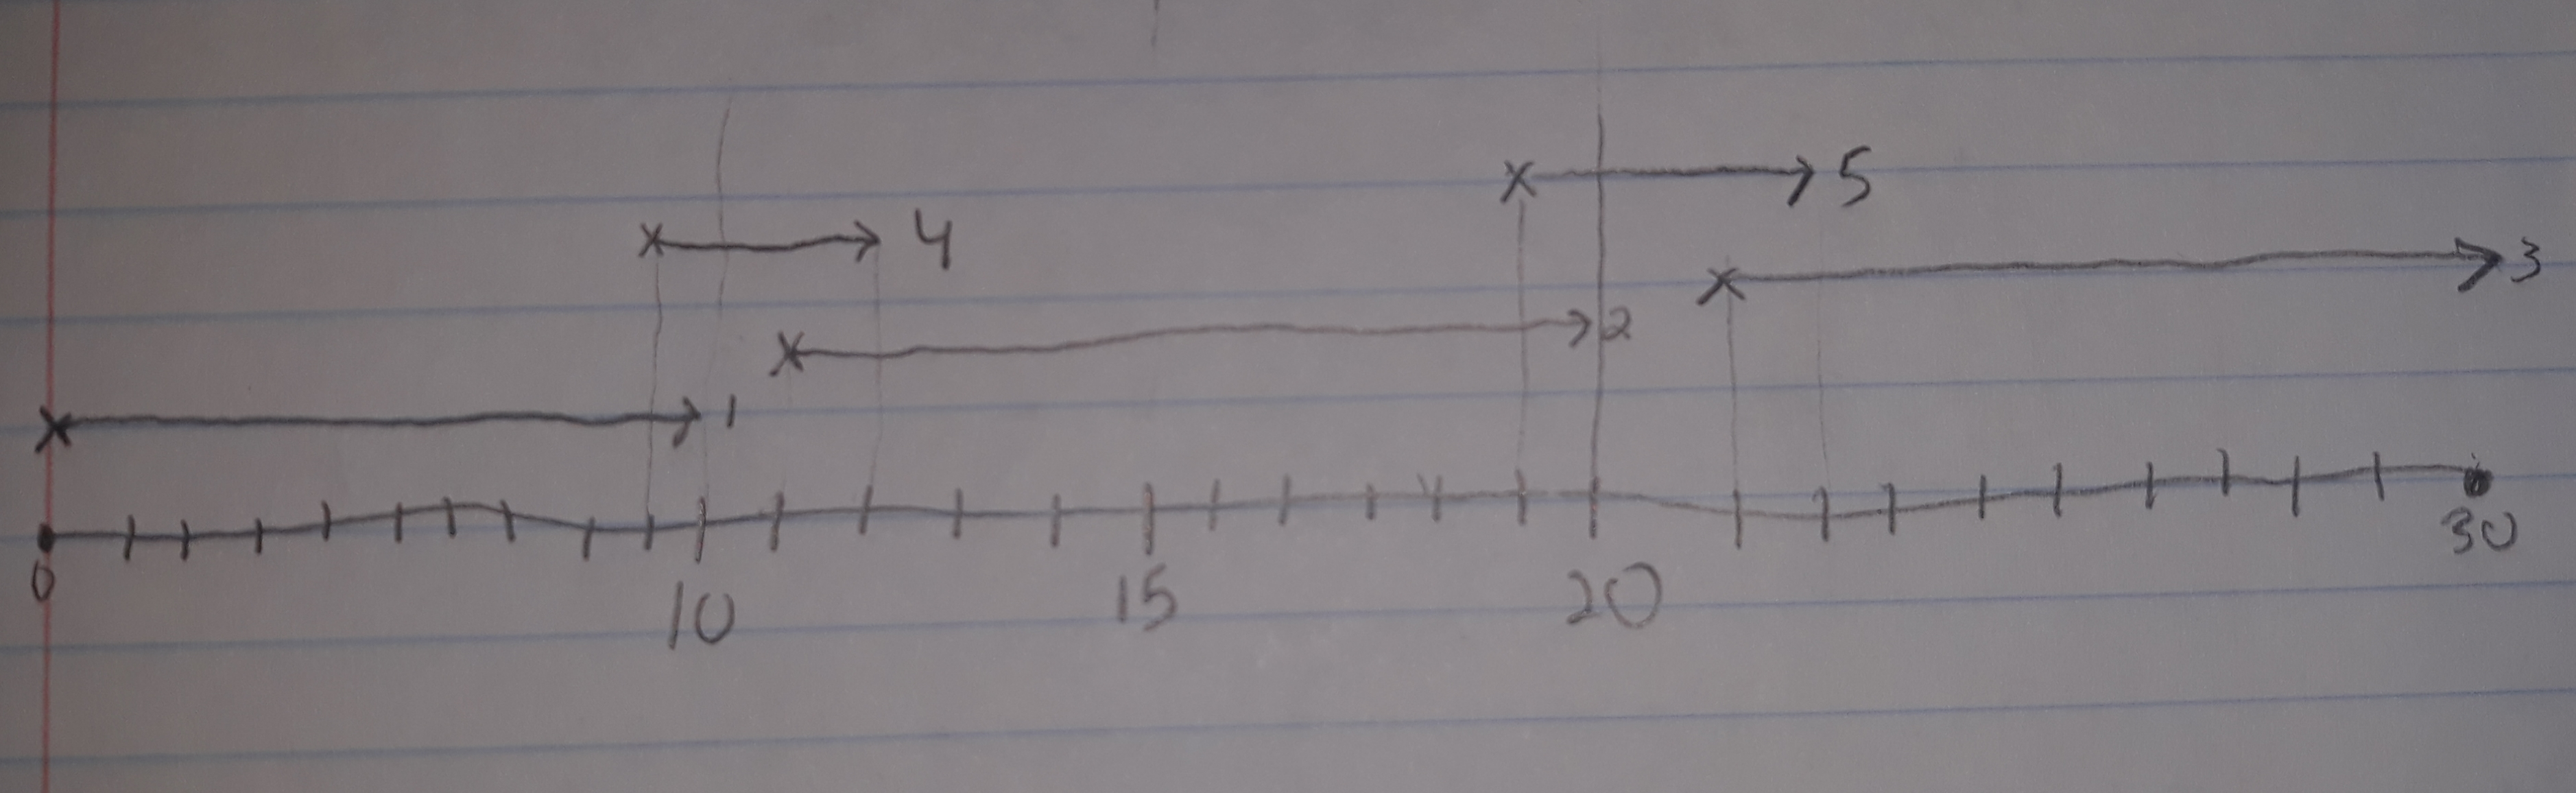
\includegraphics[width=\textwidth]{Graph2} \newline \newline$ Both events 4 and 5 overlap two separate events (1,2 and 2,3 respectively). As such, to keep a maximum amout, we discard these two events. $\newline \newline$ Therefore, the max amount of events is 3 with events (1 [1-10],2 [11-20],3 [21-30])
\end{solution}

\newpage
\item (2 pt) Suppose we sort the intervals in ascending order by interval length. For events with the same length, order by start time. Consider a greedy algorithm that selects the next interval based on the smallest interval length, so long as the interval selected does not conflict with any previously selected interval. Using the intervals provided, show that this greedy algorithm fails to provide a maximum size set of events, where no two events in the set overlap. That is, the solution returned by this greedy algorithm is not optimal.

\begin{solution}
$\newline 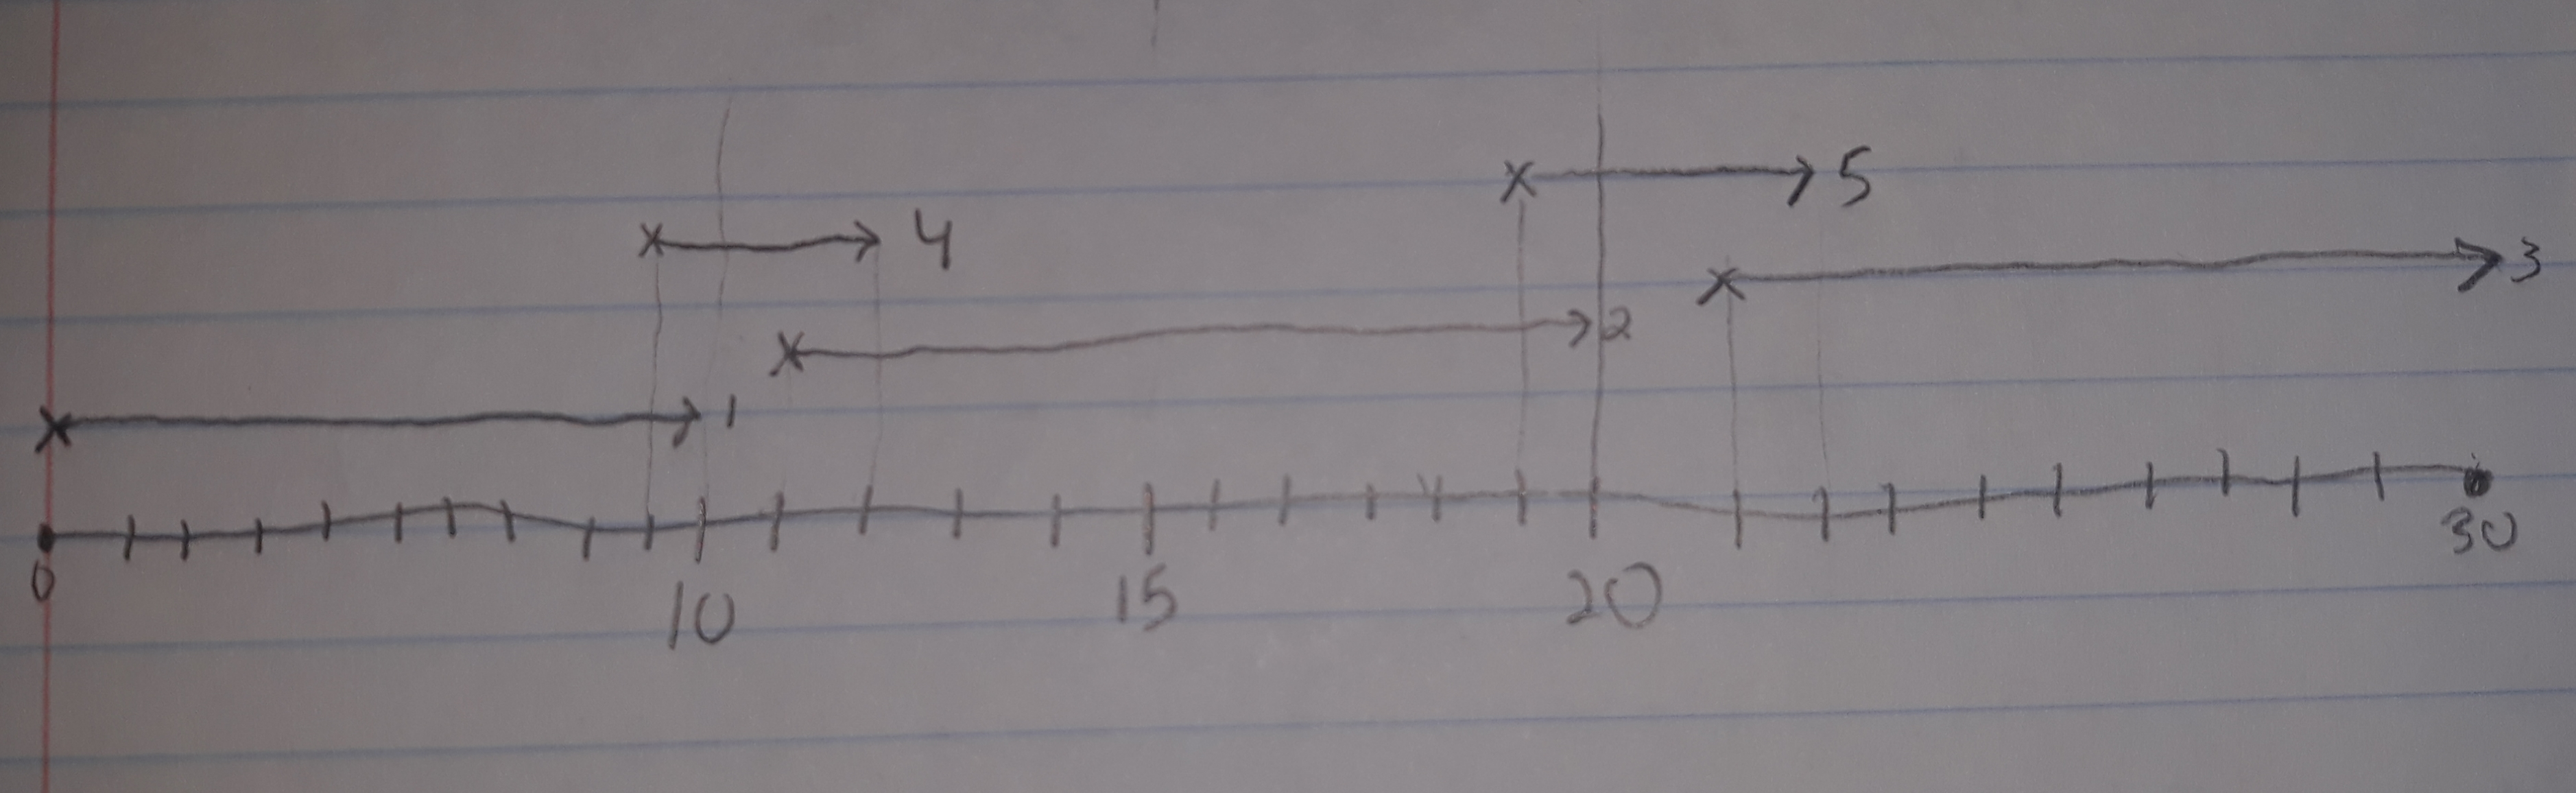
\includegraphics[width=\textwidth]{Graph2} \newline$ (copied down here for convenience) $\newline \newline$ Events 1,2,3 are 9 long, which means they have lower priority than the small 4 and 5 following the graph. $\newline$ Events 4 and 5, as the shortest non-overlapping events, are added first. These then, however, block events 1,2, and 3 from entering due overlap $\newline \newline$ Due to our algorithm, only 2 events (4,5) will be picked by size, which is less optimal than the most optimal 3 (being 1 [1-10],2 [11-20],3 [21-30])
\end{solution}

\end{enumerate}

\newpage
\item Consider again the same scenario as in Problems 1 and 2, and suppose the following intervals are provided.
\begin{center}
\begin{tabular}{c|c}
Event Index & Interval \\ \hline
1 & $[1, 3]$ \\ 
2 & $[4, 6]$ \\
3 & $[7, 9]$ \\
4 & $[10, 12]$ \\
5 & $[2, 5]$ \\
6 & $[2, 5]$ \\
7 & $[2, 5]$ \\
8 & $[5.5, 7.5]$ \\
9 & $[8, 11]$ \\
10 & $[8, 11]$ \\
11 & $[8, 11]$ \\
\end{tabular}
\end{center}

\begin{enumerate}[label=(\alph*)]
\item  (1 pt) What is the maximum size set of events that can be selected such that no two events in the set overlap? Include the list of the events selected in your answer.
\begin{solution}
$\pagebreak \newline 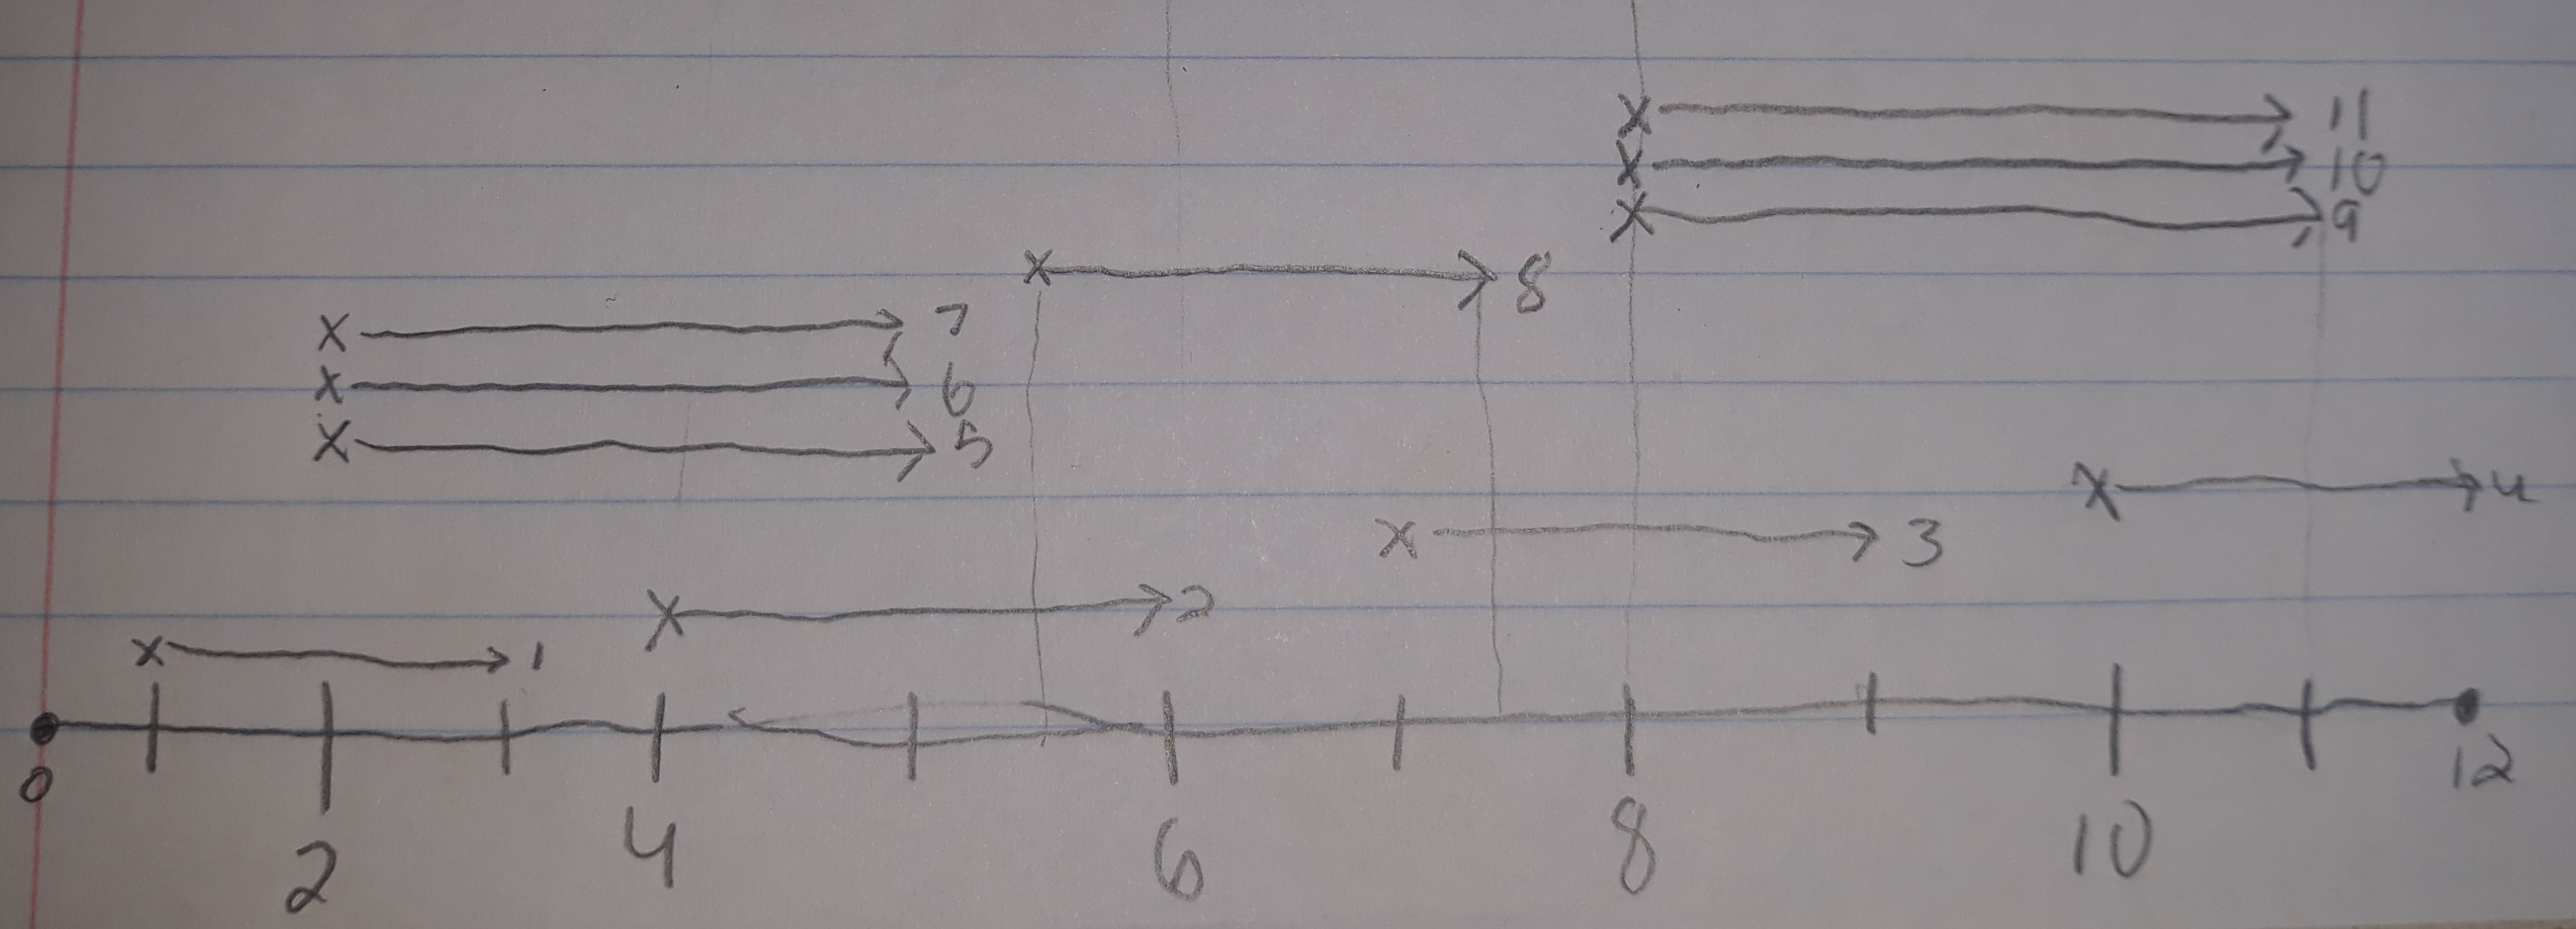
\includegraphics[width=\textwidth]{Graph3} \newline \newline$ To start, there are two sets that are the exact same value ((5,6,7) and (9,10,11)), which automatically overlap and thus will be counted as one entity. $\newline$ Following the graph, we have another situation like question 2 where there are lines at the bottom that correctly fit the whole linespace and others that overlap two simultaneously, eliminating two (such as the events 5,6,7 conglomerate taking over what could fit both events 1 and 2). As such, every line besides 1,2,3,4 overlaps two separate lines (not including the ones with the same value)  and thus should be ignored for optimality $\newline \newline$ As such, the max amount of events is 4 with the events (1 [1-3],2 [4-6],3 [7-9],4 [10-12]).
\end{solution}

\newpage
\item (2 pts) Let $c_{i}$ denote the number of intervals on our list in which interval $i$ conflicts. For example, interval $1$ participates in $3$ conflicts: with intervals $5, 6,$ and $7$. So $c_{1} = 3$. \\

\noindent Suppose we sort the intervals in ascending order based on the number of conflicts. So if $c_{i} < c_{j}$, then interval $i$ comes before interval $j$. Consider a greedy algorithm that selects the next interval based on the smallest number of conflicts, so long as the interval selected does not conflict with any previously selected interval. Using the intervals provided, show that this greedy algorithm fails to provide a maximum size set of events, where no two events in the set overlap. That is, the solution returned by this greedy algorithm is not optimal.
\end{enumerate}

\begin{solution}
$\pagebreak \newline 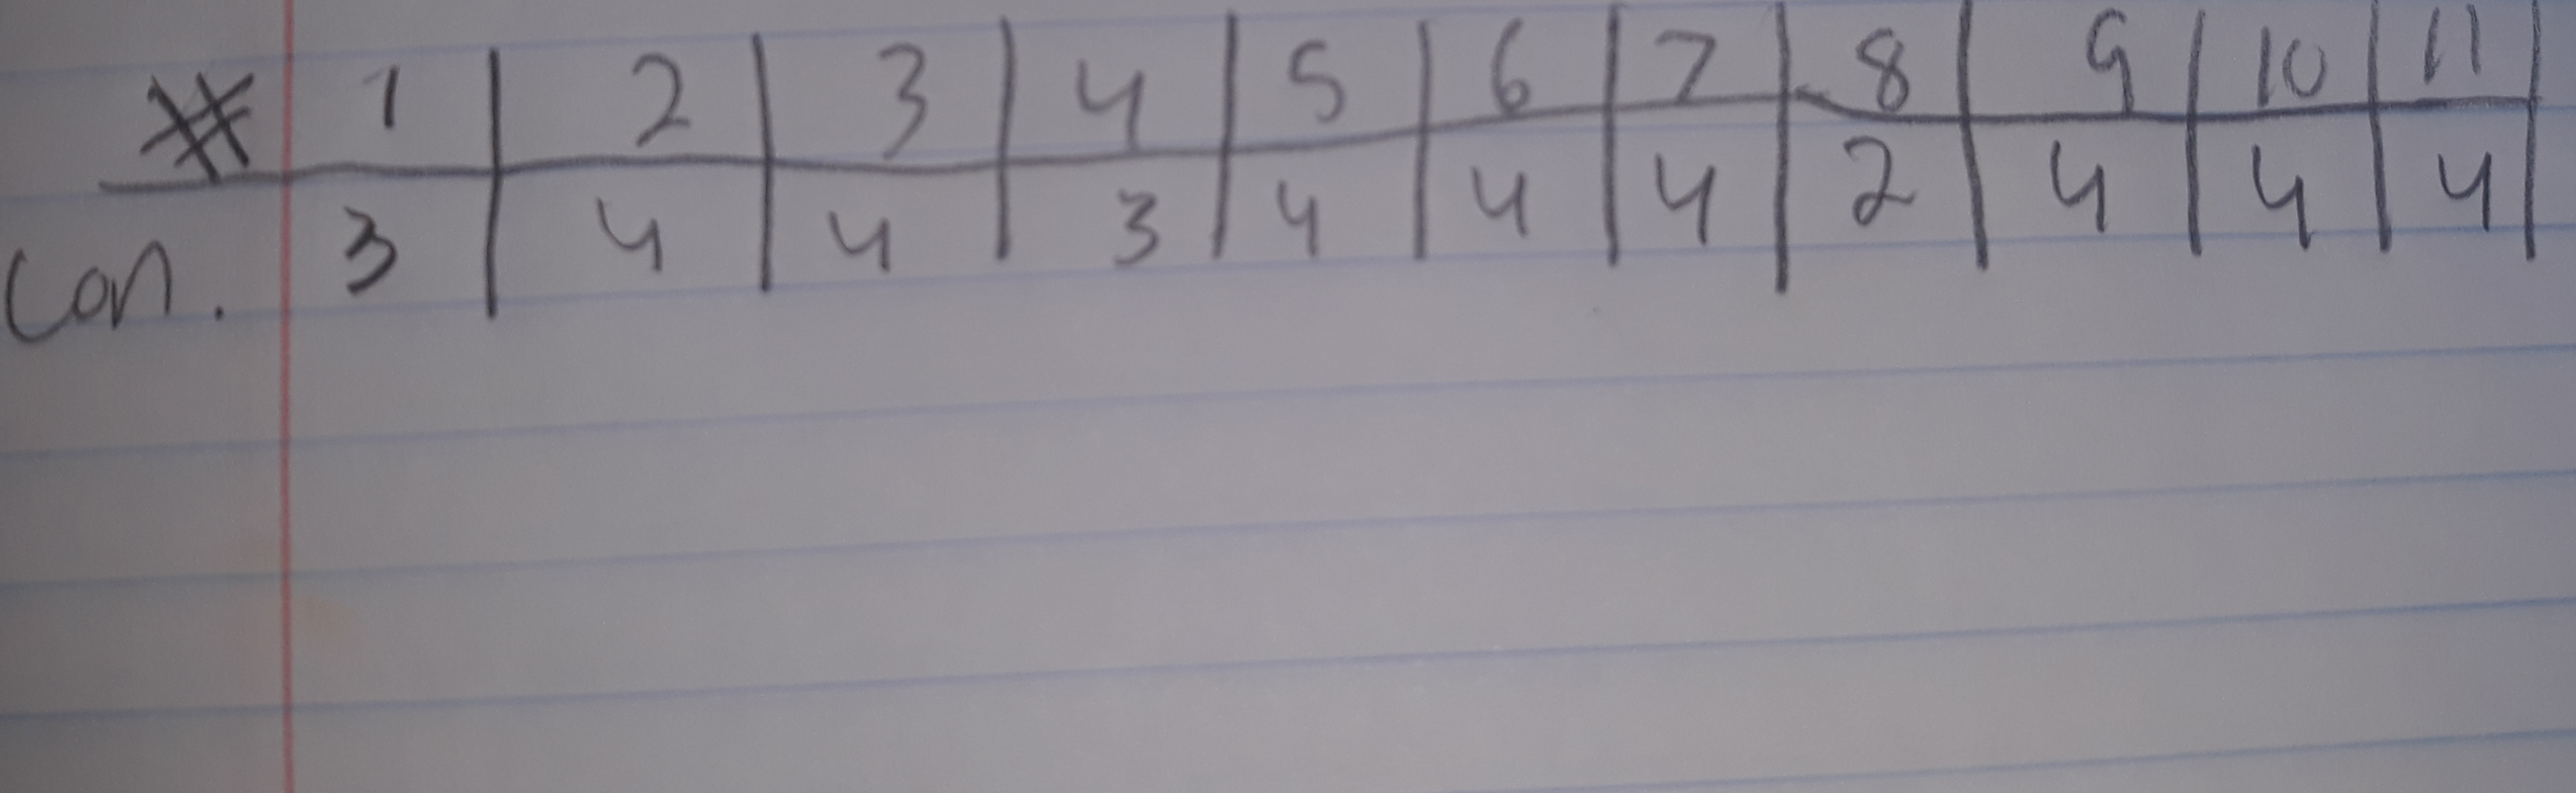
\includegraphics[width=\textwidth]{Graph4} \newline$ $\#$ is the event number, con is the number of conflicts $\newline 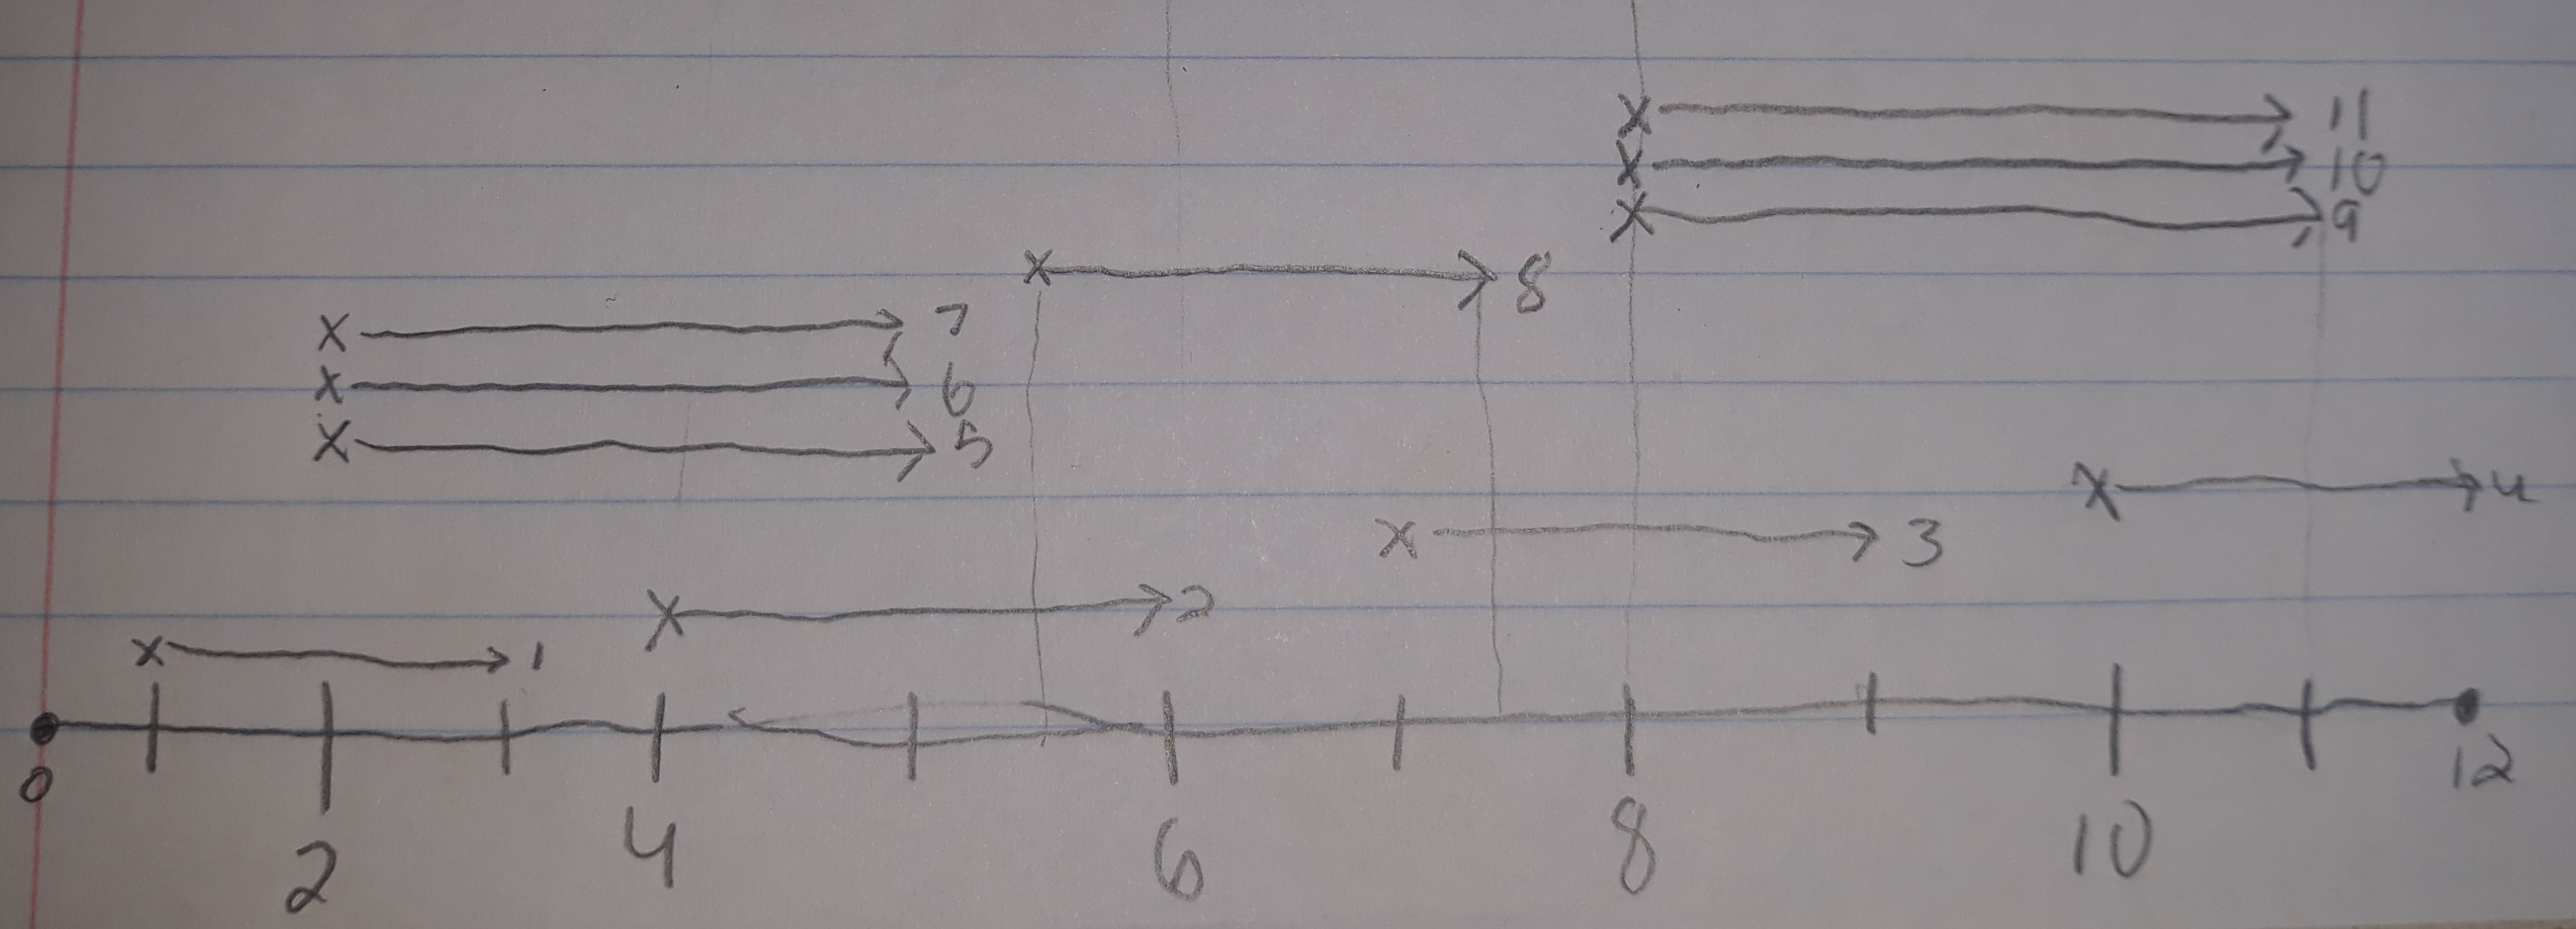
\includegraphics[width=\textwidth]{Graph3} \newline$ (copied down here for convenience) $\newline \newline$ According to our chart of conflicts, to follow the rules, event 8 would be picked first as the only one with only two conflicts. 1 and 4 would follow, as they are the only ones with 3 conflicts while also not conflicting with 8. All others conflict with 8,1, and/or 4 $\newline \newline$ Since 8 is being used, we cannot use the most optimal 2 and 3 with our picked 1 and 4, leading to 3 events instead of 4, thus being not as optimal. 
\end{solution}


\end{enumerate}

\end{document}


